\chapter*{Abstract}

\chapter{Introduction}
\begin{itemize}
  \item gene expression is noisy, same cells end up different \cite{elowitz2002}
  \item why it matters: HIV latency, persisters, cancer drug resistance
  \begin{itemize}
    \item lead with HIV since that's the data
  \end{itemize}
  \item can't see the rates directly, only fluorescence
  \item goal: get the rates back from the movies
  \begin{itemize}
    \item list the 4 goals from the proposal, then say what actually happened
  \end{itemize}
\end{itemize}

\chapter{Background and Theory}

\section{Chemical reaction networks and the Gillespie algorithm}
\begin{itemize}
  \item reactions + rates, pick when and which \cite{wilkinson2019}
  \begin{itemize}
    \item probably need the master equation here, just one line
  \end{itemize}
\end{itemize}

\section{Two models of gene expression}
\begin{itemize}
  \item birth-death, Poisson steady state
  \item telegraph model, promoter on/off, exact distribution \cite{peccoud1995}
  \begin{itemize}
    \item copy the P(n) formula from week 2
  \end{itemize}
  \item burst frequency $k_{on}$, burst size $k_m/k_{off}$
\end{itemize}

\section{Approximate Bayesian computation}
\begin{itemize}
  \item no likelihood so simulate and compare summary stats
  \item regression adjustment \cite{beaumont2002}
  \item coverage test
  \begin{itemize}
    \item explain the p(theta | s(y)) thing, stats lose info
  \end{itemize}
\end{itemize}

\section{Particle filtering}
\begin{itemize}
  \item propagate, weight, resample
\end{itemize}

\chapter{Data}
\begin{itemize}
  \item Dar lab HIV screen \cite{lu2021,idb_dataset}, one well (K16)
  \begin{itemize}
    \item say why only one well (download size)
  \end{itemize}
  \item Cellpose \cite{stringer2021} + Hungarian tracking
  \begin{itemize}
    \item check if I actually handle cell division before saying so
  \end{itemize}
  \item 479 cells, 72 frames
  \item background + drift
\end{itemize}

\begin{figure}[htbp]\centering
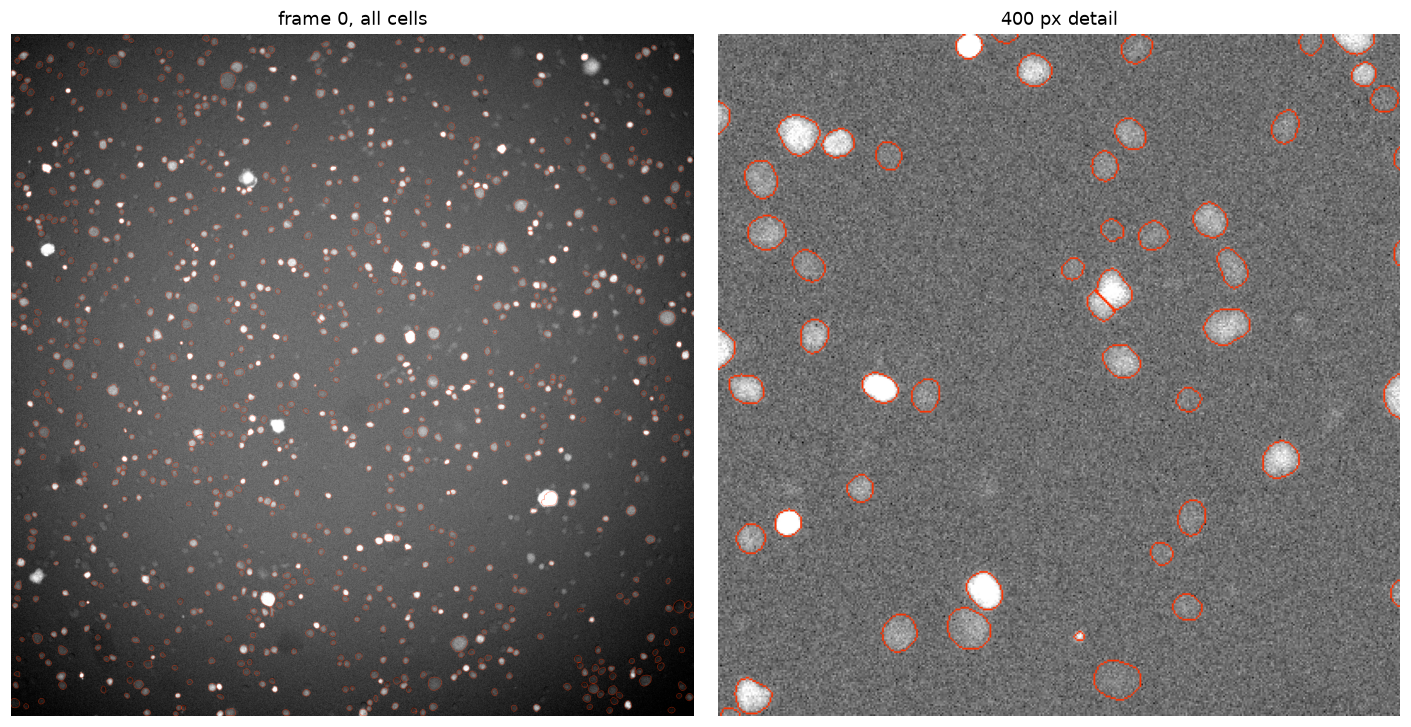
\includegraphics[width=0.6\linewidth]{figures/segmentation_overlay.png}
\caption{Segmentation.}
\end{figure}

\begin{figure}[htbp]\centering
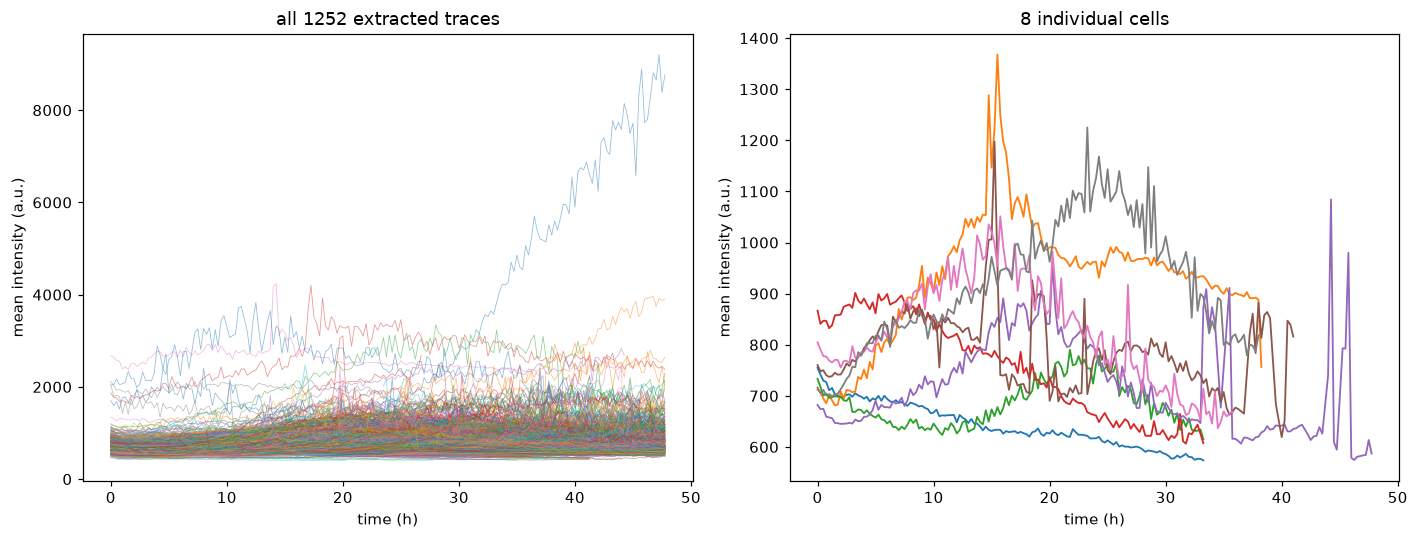
\includegraphics[width=0.85\linewidth]{figures/extracted_traces.png}
\caption{Extracted traces.}
\end{figure}

\begin{figure}[htbp]\centering
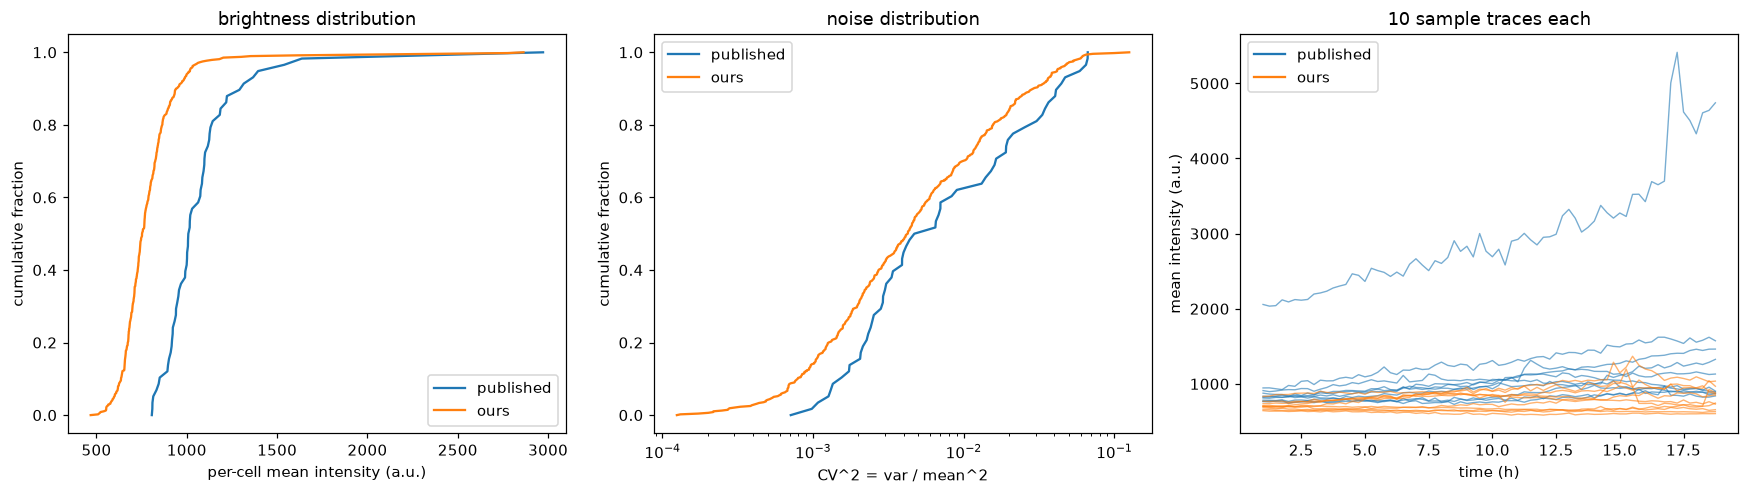
\includegraphics[width=0.85\linewidth]{figures/comparison_with_published.png}
\caption{Mine vs published traces.}
\end{figure}

\begin{figure}[htbp]\centering
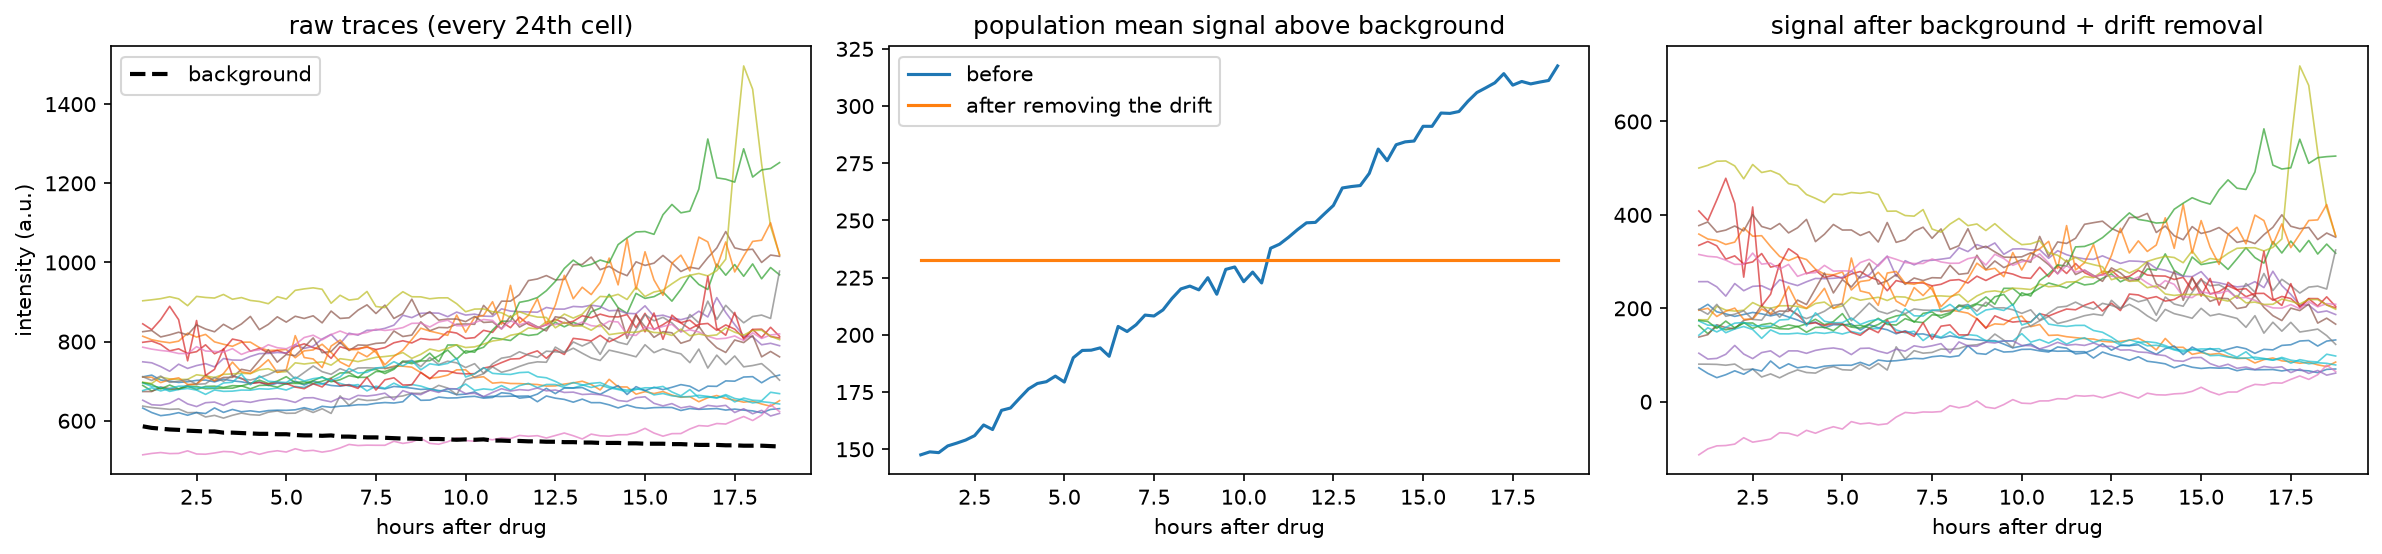
\includegraphics[width=\linewidth]{figures/week4_traces_background_drift.png}
\caption{Background and drift.}
\end{figure}

\chapter{Methods and Validation}

\section{Stochastic simulator}
\begin{itemize}
  \item one gillespie function for both models
  \item checks against exact answers
  \item can't vectorise it, each step depends on the last
\end{itemize}

\begin{figure}[htbp]\centering
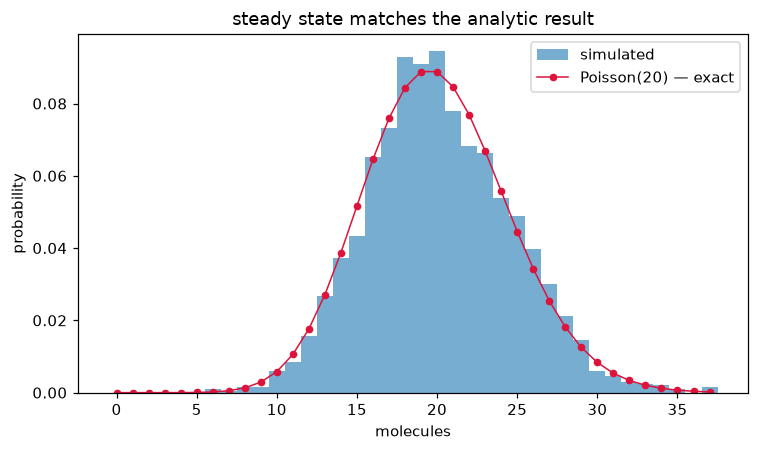
\includegraphics[width=0.6\linewidth]{figures/week2_birth_death_distribution.png}
\caption{Birth-death vs Poisson.}
\end{figure}

\begin{figure}[htbp]\centering
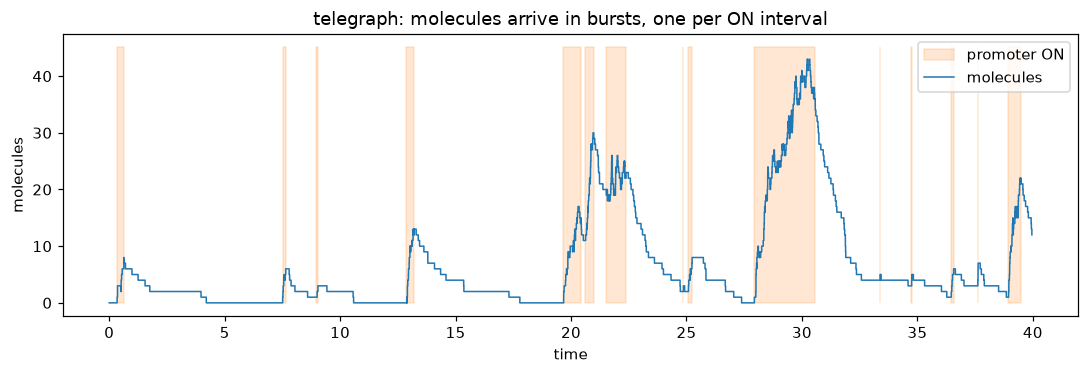
\includegraphics[width=0.85\linewidth]{figures/week2_telegraph_trajectory.png}
\caption{Telegraph trajectory.}
\end{figure}

\begin{figure}[htbp]\centering
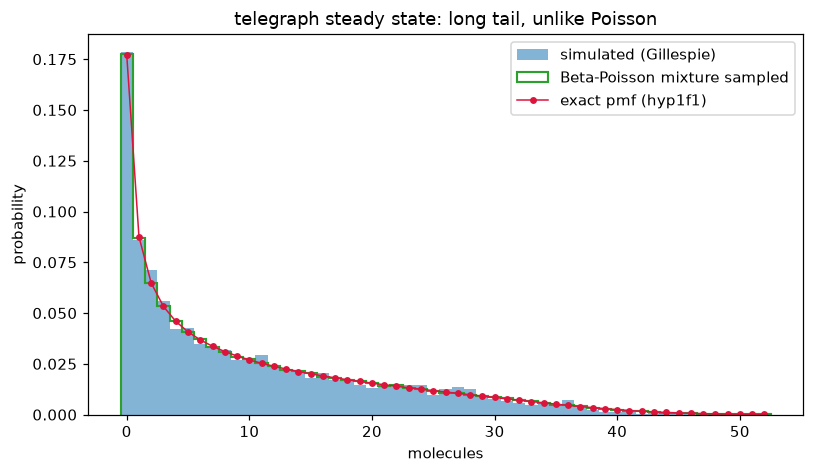
\includegraphics[width=0.6\linewidth]{figures/week2_telegraph_distribution.png}
\caption{Telegraph vs exact.}
\end{figure}

\begin{figure}[htbp]\centering
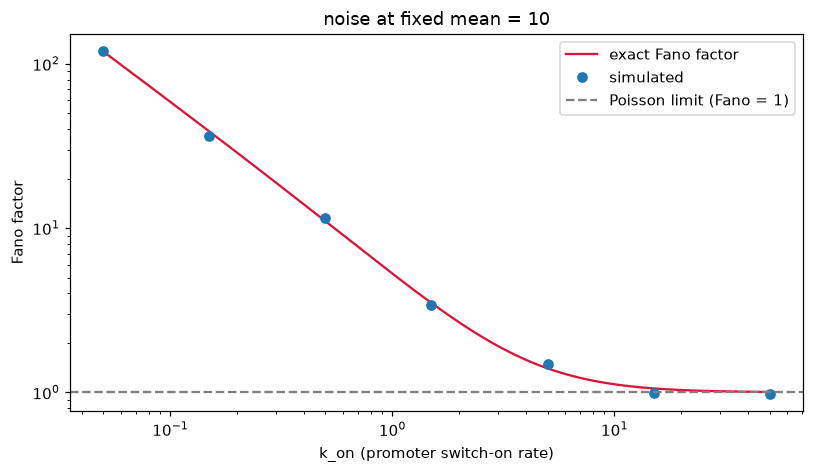
\includegraphics[width=0.6\linewidth]{figures/week2_noise_vs_switching.png}
\caption{Fano factor vs $k_{on}$.}
\end{figure}

\section{ABC on synthetic data}
\begin{itemize}
  \item 10 cells, 50 frames, keep closest 1\%
  \item gets true values back but $k_{off}$ is wide
\end{itemize}

\begin{figure}[htbp]\centering
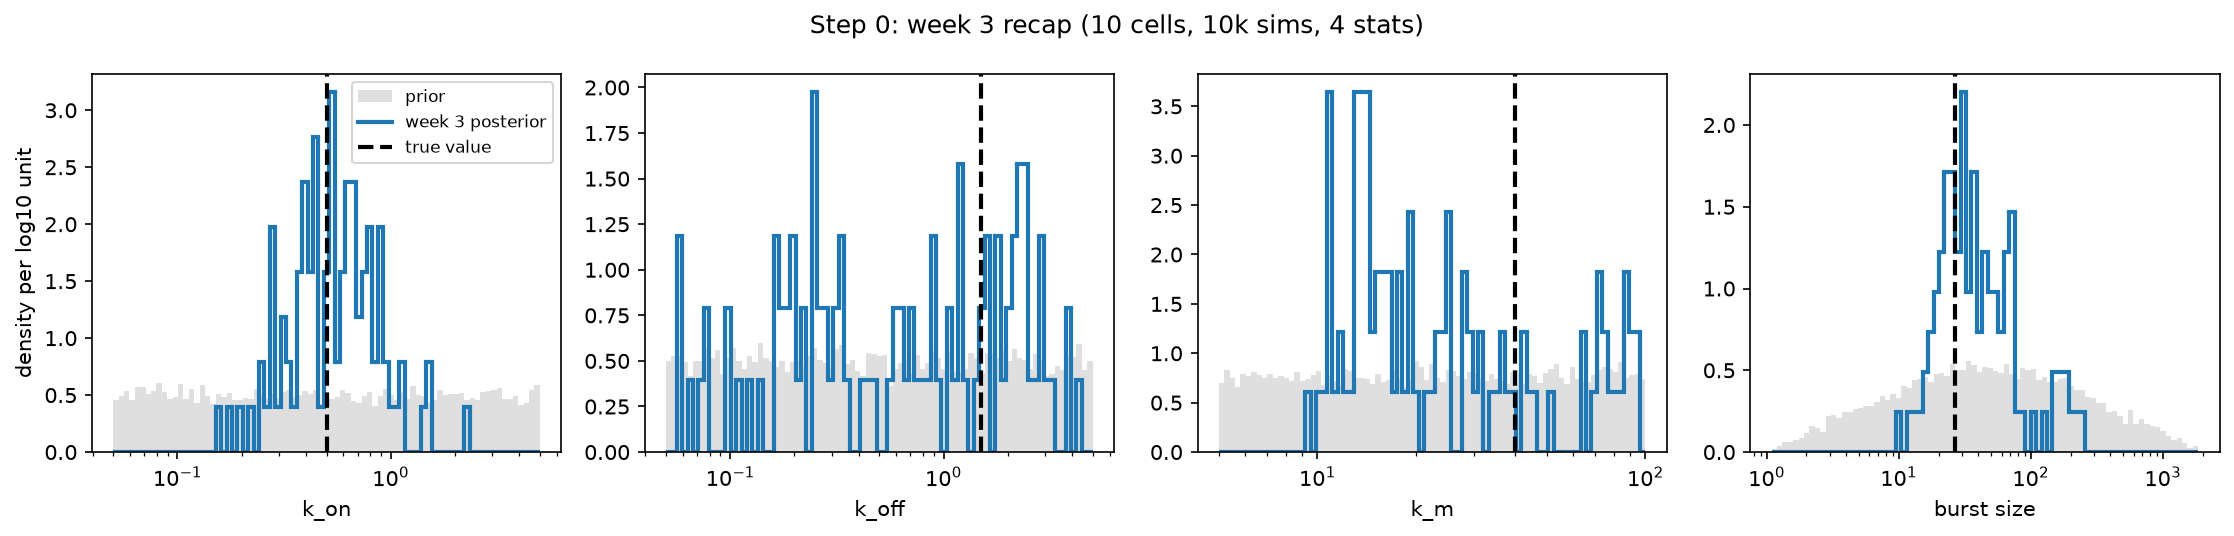
\includegraphics[width=\linewidth]{figures/week3_5_figure0_posterior.png}
\caption{Week 3 posterior.}
\end{figure}

\begin{figure}[htbp]\centering
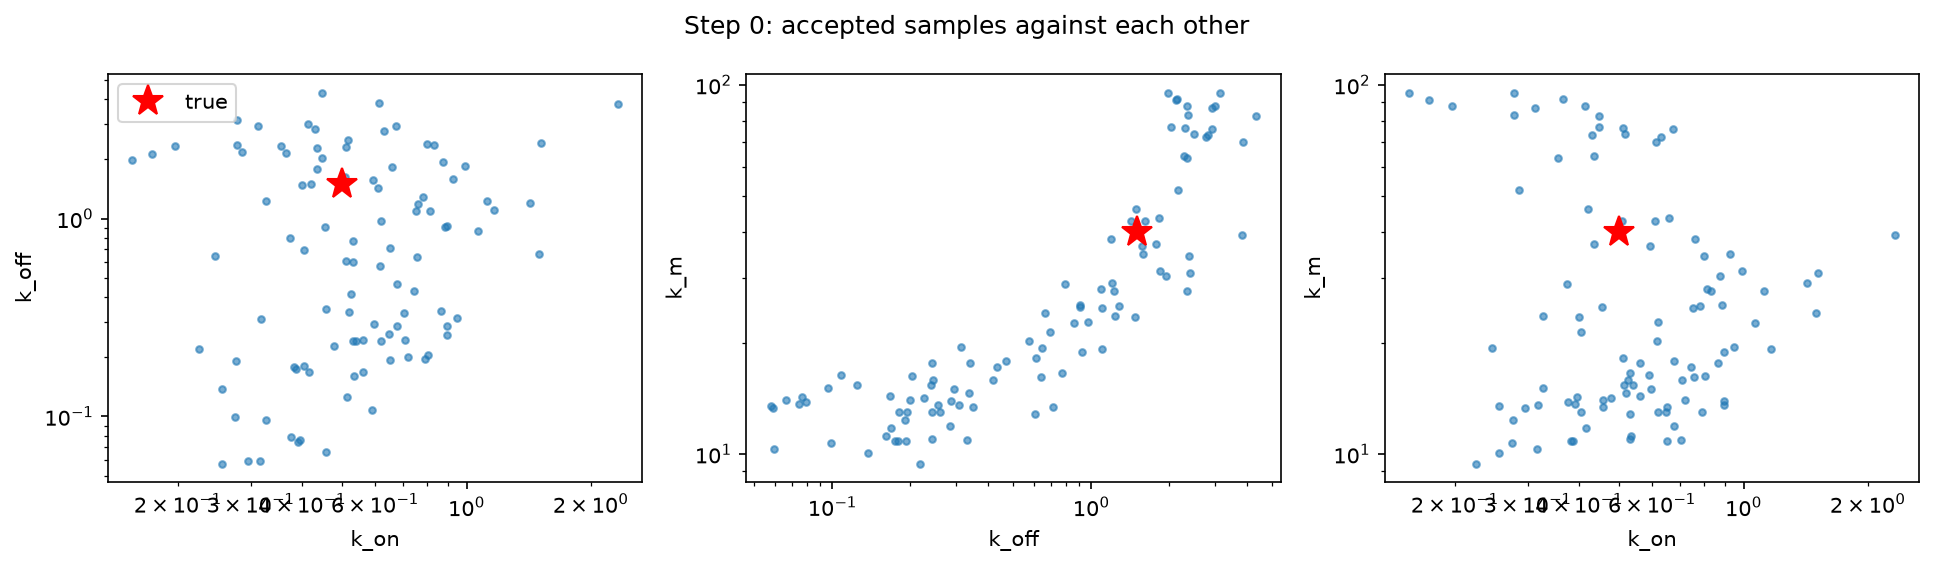
\includegraphics[width=\linewidth]{figures/week3_5_figure0_pairs.png}
\caption{Accepted samples.}
\end{figure}

\section{Why were the intervals wide?}
\begin{itemize}
  \item more cells
  \item more stats + regression adjustment
  \item exact likelihood to compare
  \begin{itemize}
    \item this is the key result for this section, exact is way narrower than rejection
  \end{itemize}
  \item coverage test
  \item EC2 for the 100k sims
\end{itemize}

\begin{figure}[htbp]\centering
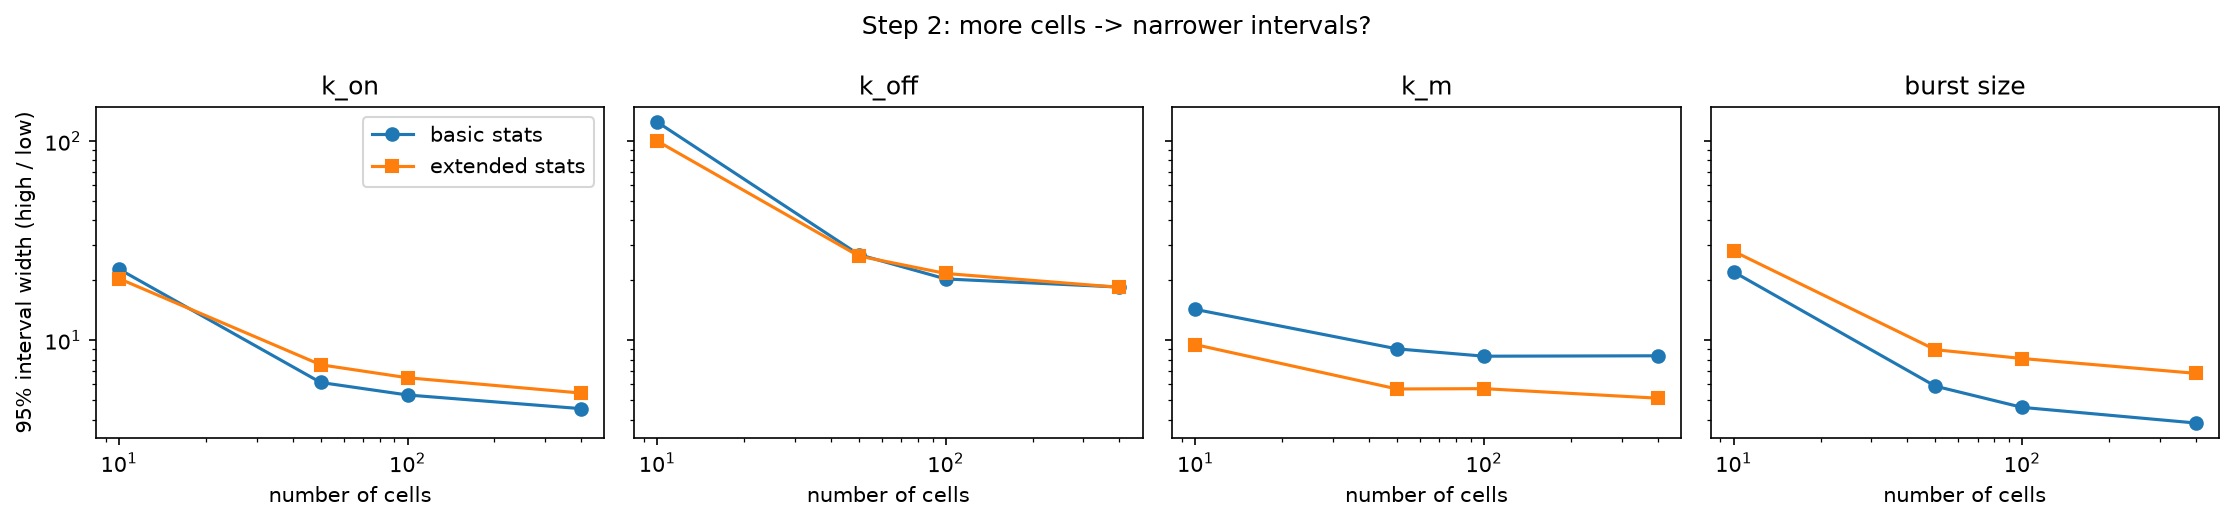
\includegraphics[width=\linewidth]{figures/week3_5_figure2_n_cells.png}
\caption{Number of cells.}
\end{figure}

\begin{figure}[htbp]\centering
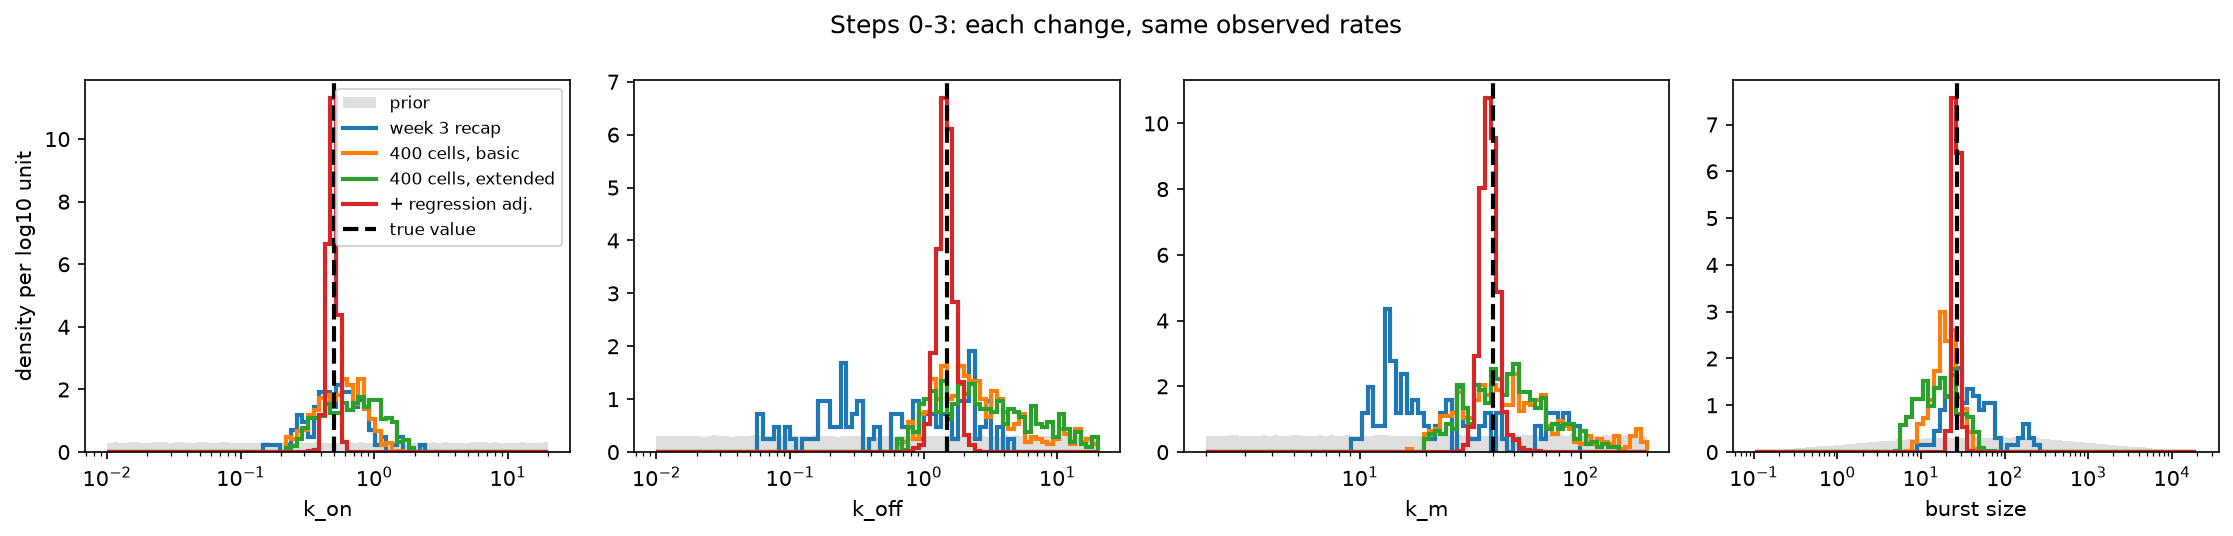
\includegraphics[width=\linewidth]{figures/week3_5_figure3_posteriors.png}
\caption{Each change.}
\end{figure}

\begin{figure}[htbp]\centering
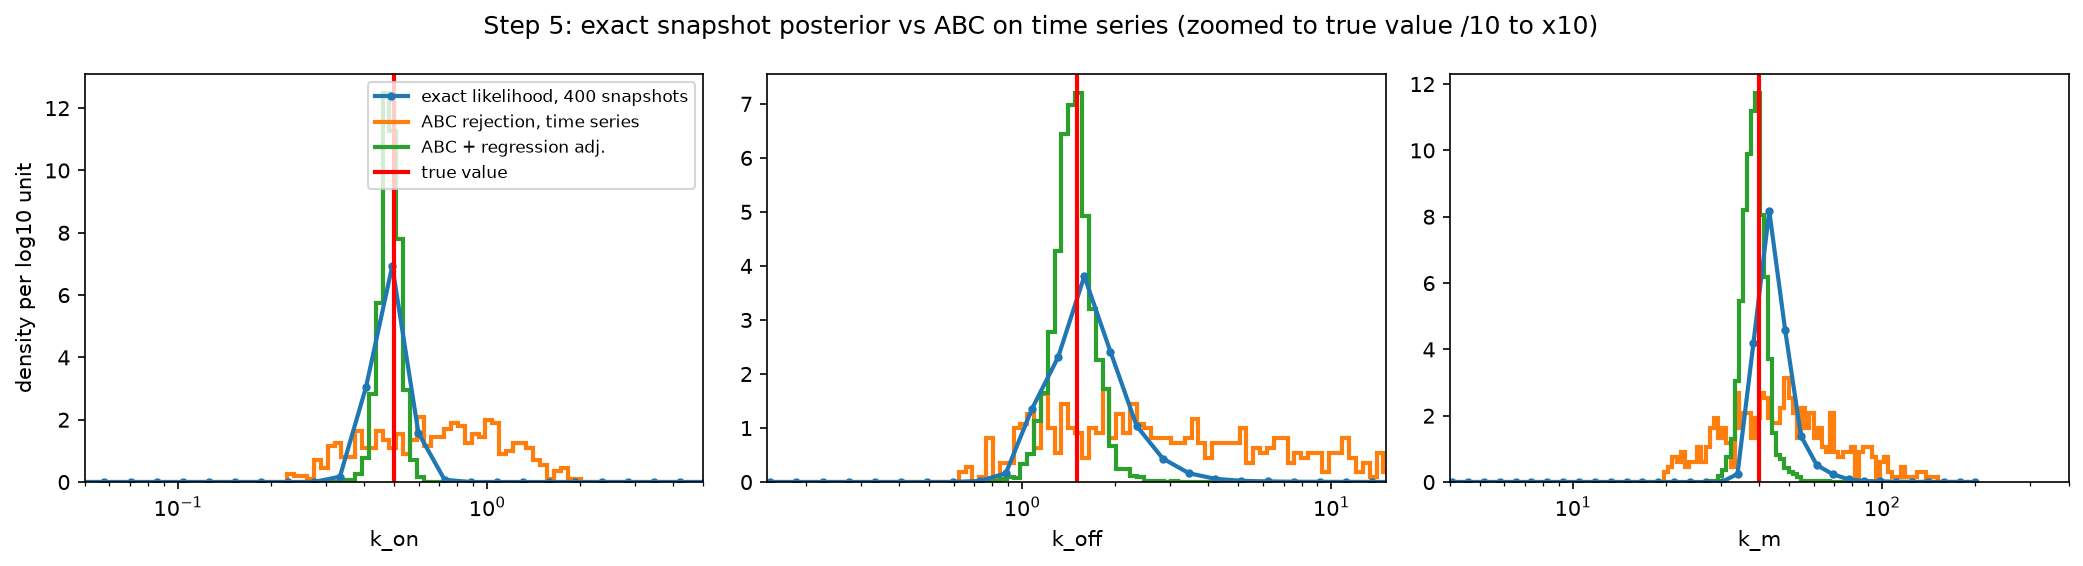
\includegraphics[width=\linewidth]{figures/week3_5_figure5_exact_likelihood.png}
\caption{Exact likelihood vs ABC.}
\end{figure}

\begin{figure}[htbp]\centering
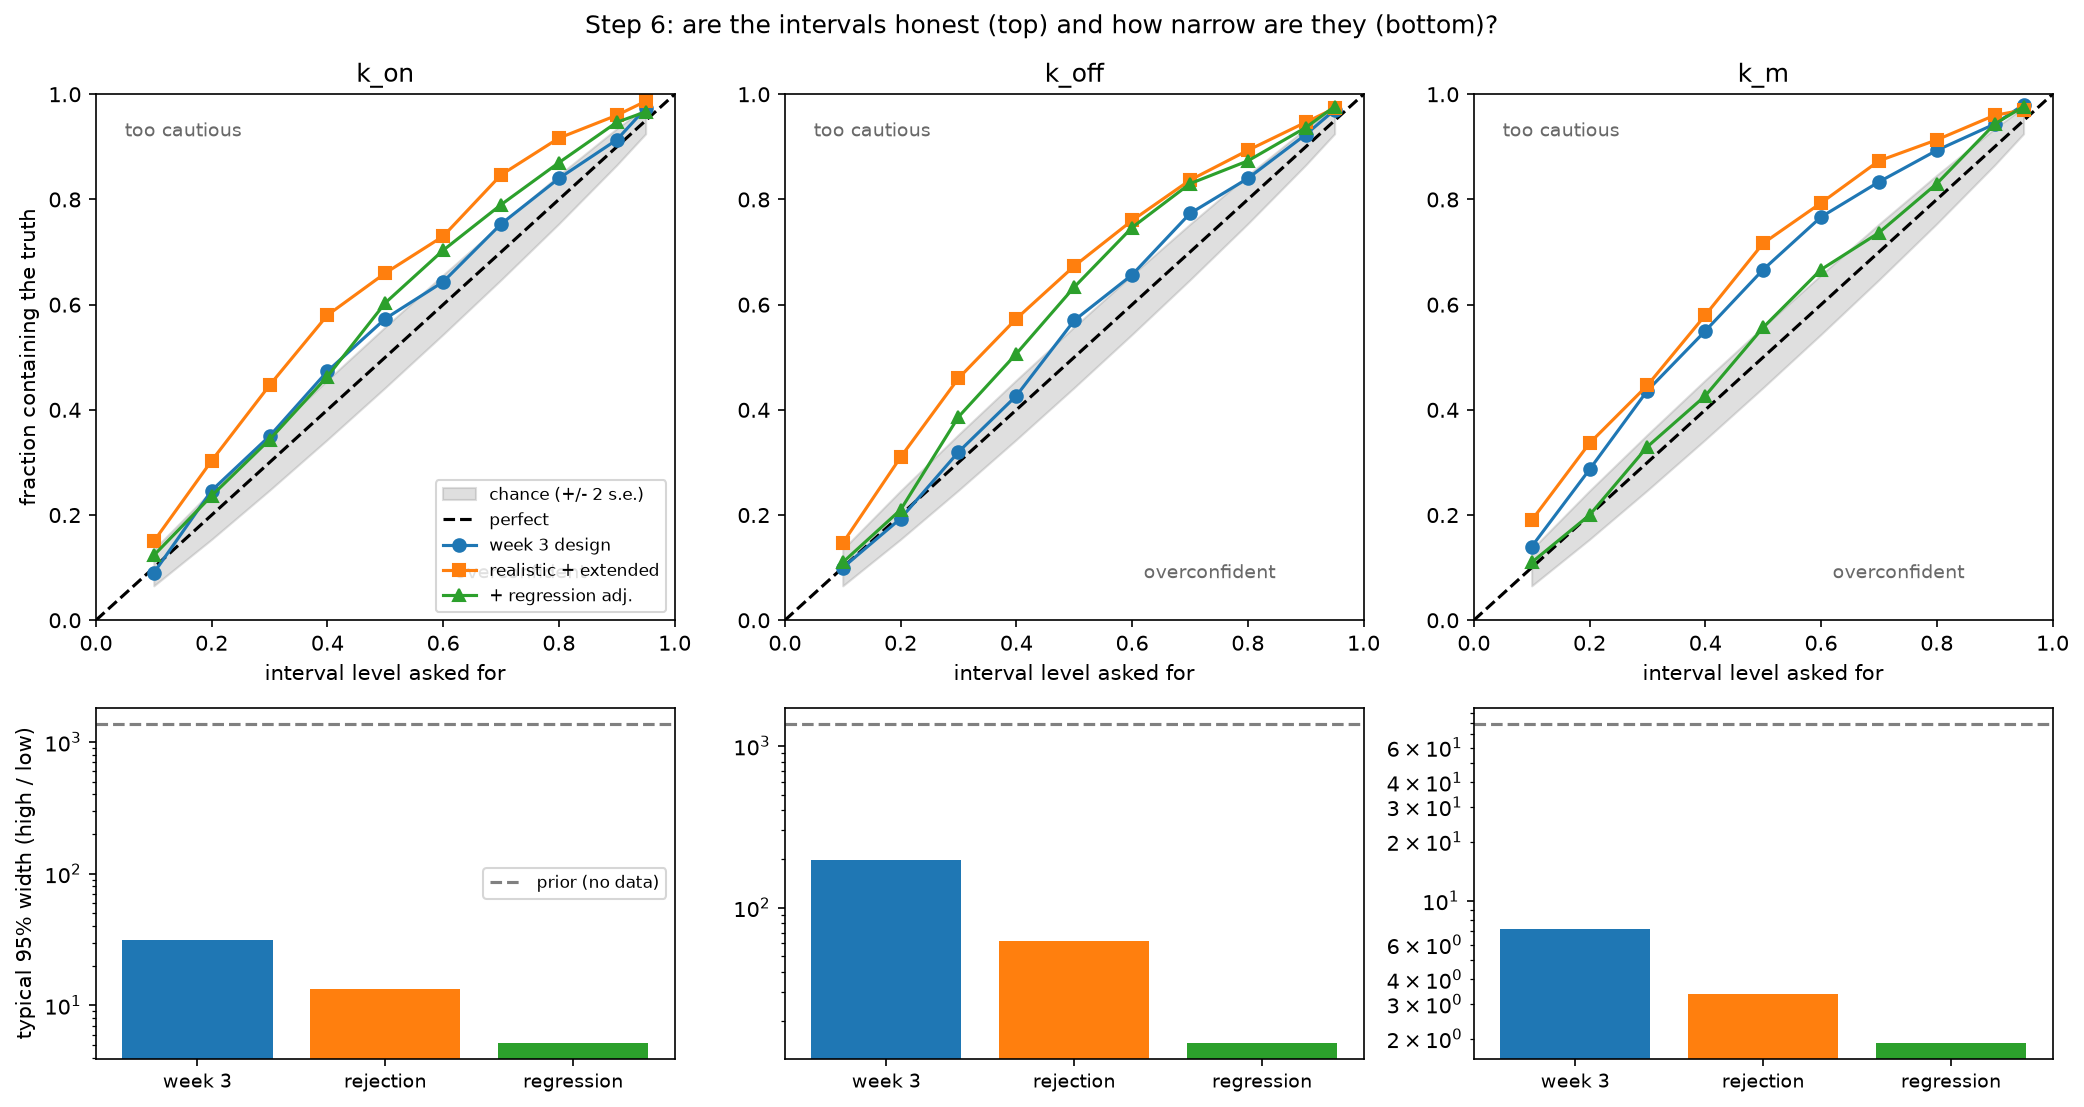
\includegraphics[width=\linewidth]{figures/week3_5_figure6_coverage.png}
\caption{Coverage.}
\end{figure}

\begin{figure}[htbp]\centering
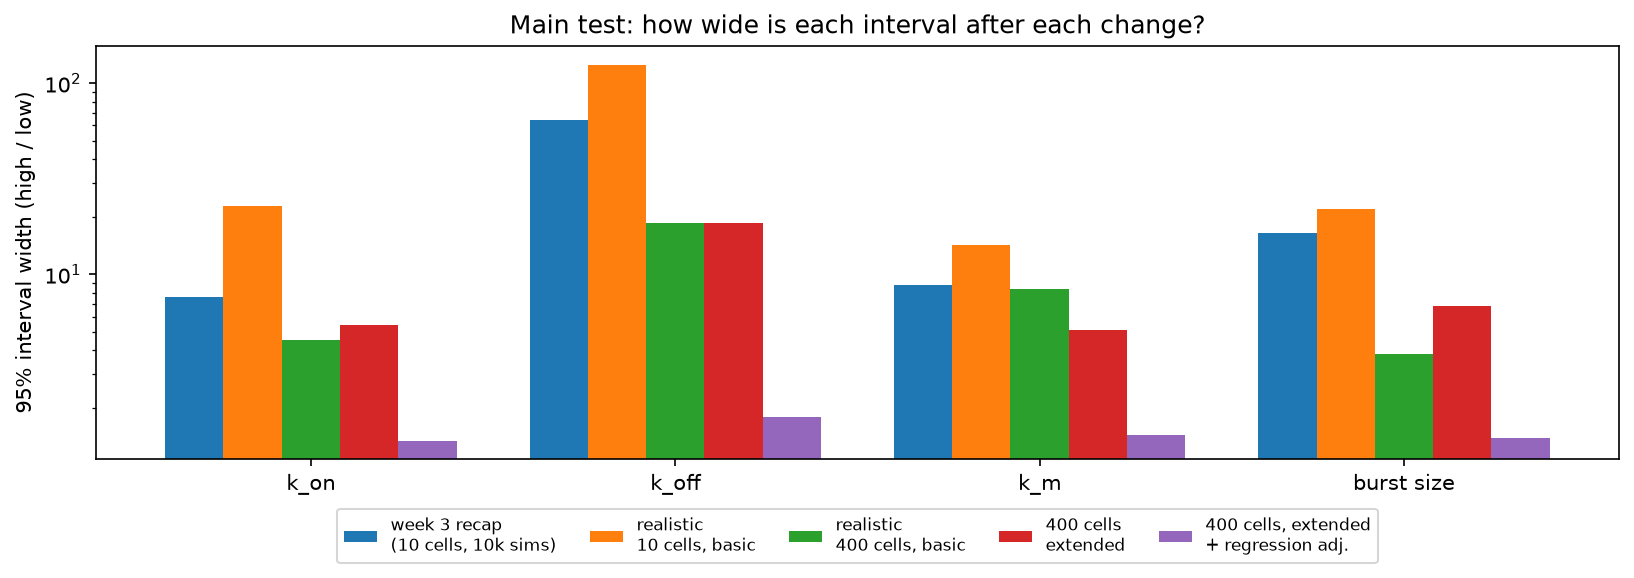
\includegraphics[width=\linewidth]{figures/week3_5_interval_widths.png}
\caption{Interval widths.}
\end{figure}

\section{Model for the real data}
\begin{itemize}
  \item large number model, extra params $A$, $\sigma$, $\eta$
  \item checked against Gillespie
  \begin{itemize}
    \item maybe a small table instead of a figure
  \end{itemize}
\end{itemize}

\chapter{Results on the HIV Circuit}

\section{Posterior}
\begin{itemize}
  \item redo coverage first
  \item burst freq ~0.5/h, eta ~0.6
  \begin{itemize}
    \item burst size only in a.u., say this early
  \end{itemize}
\end{itemize}

\begin{figure}[htbp]\centering
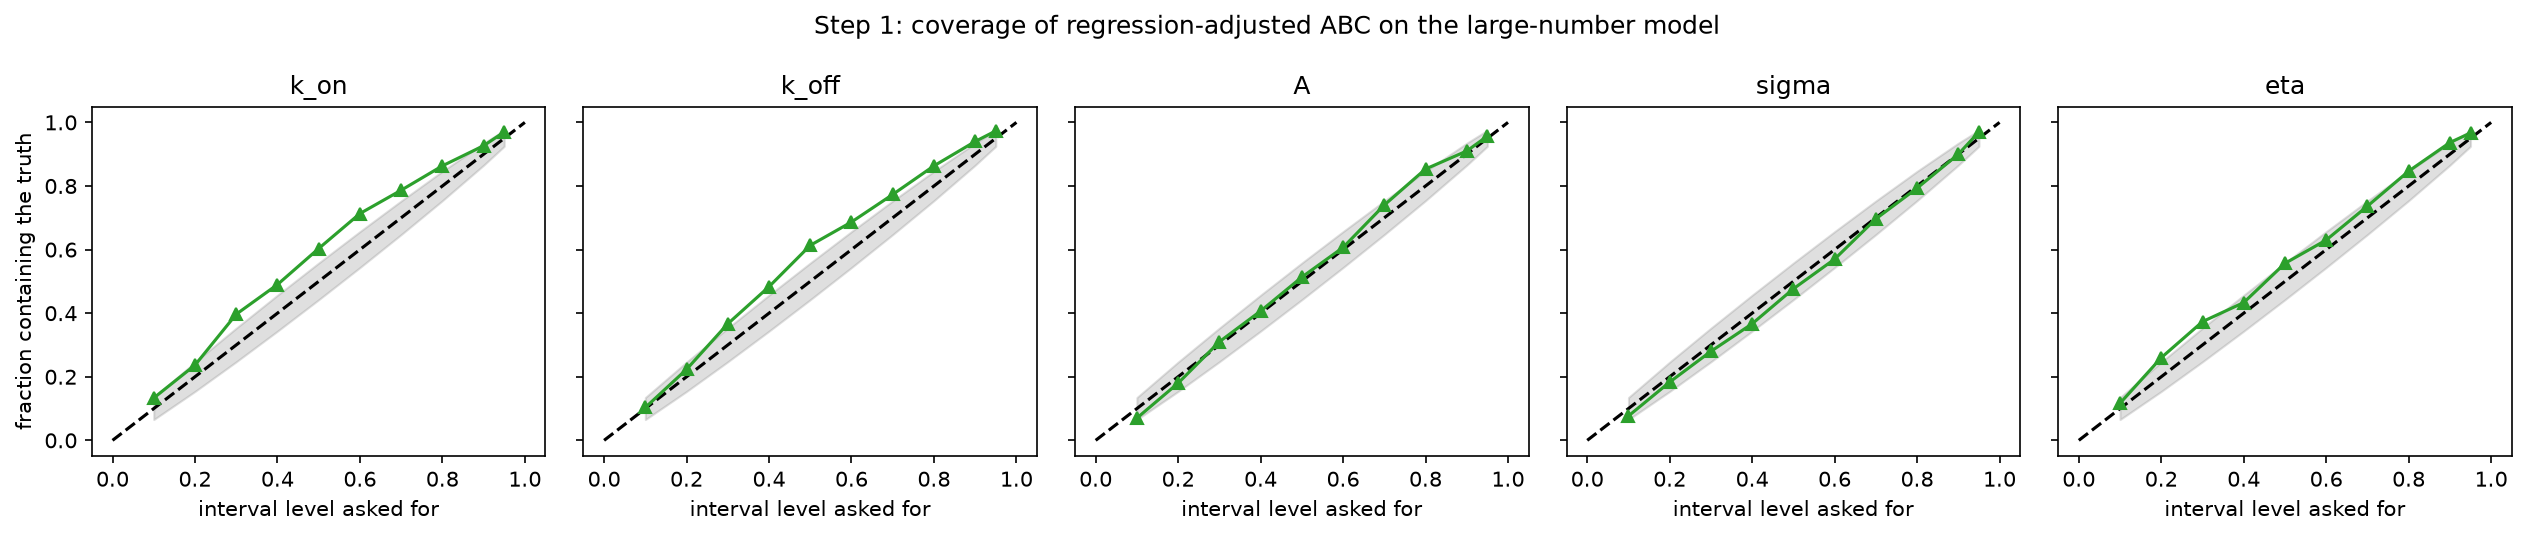
\includegraphics[width=\linewidth]{figures/week4_figure1_coverage.png}
\caption{Coverage on new model.}
\end{figure}

\begin{figure}[htbp]\centering
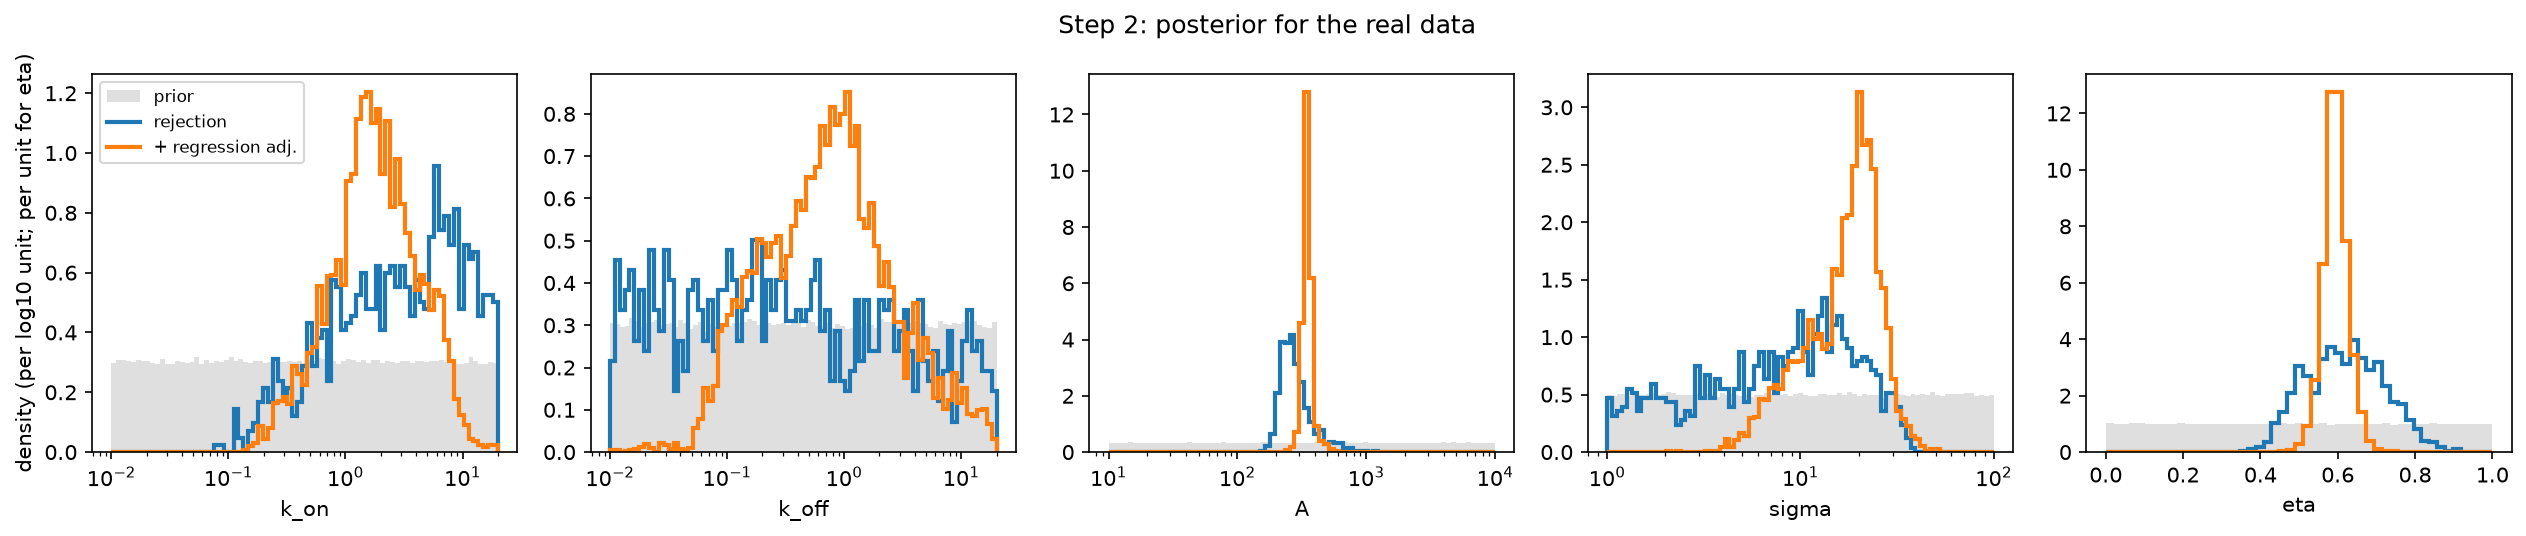
\includegraphics[width=\linewidth]{figures/week4_figure2_posterior.png}
\caption{Real data posterior.}
\end{figure}

\begin{figure}[htbp]\centering
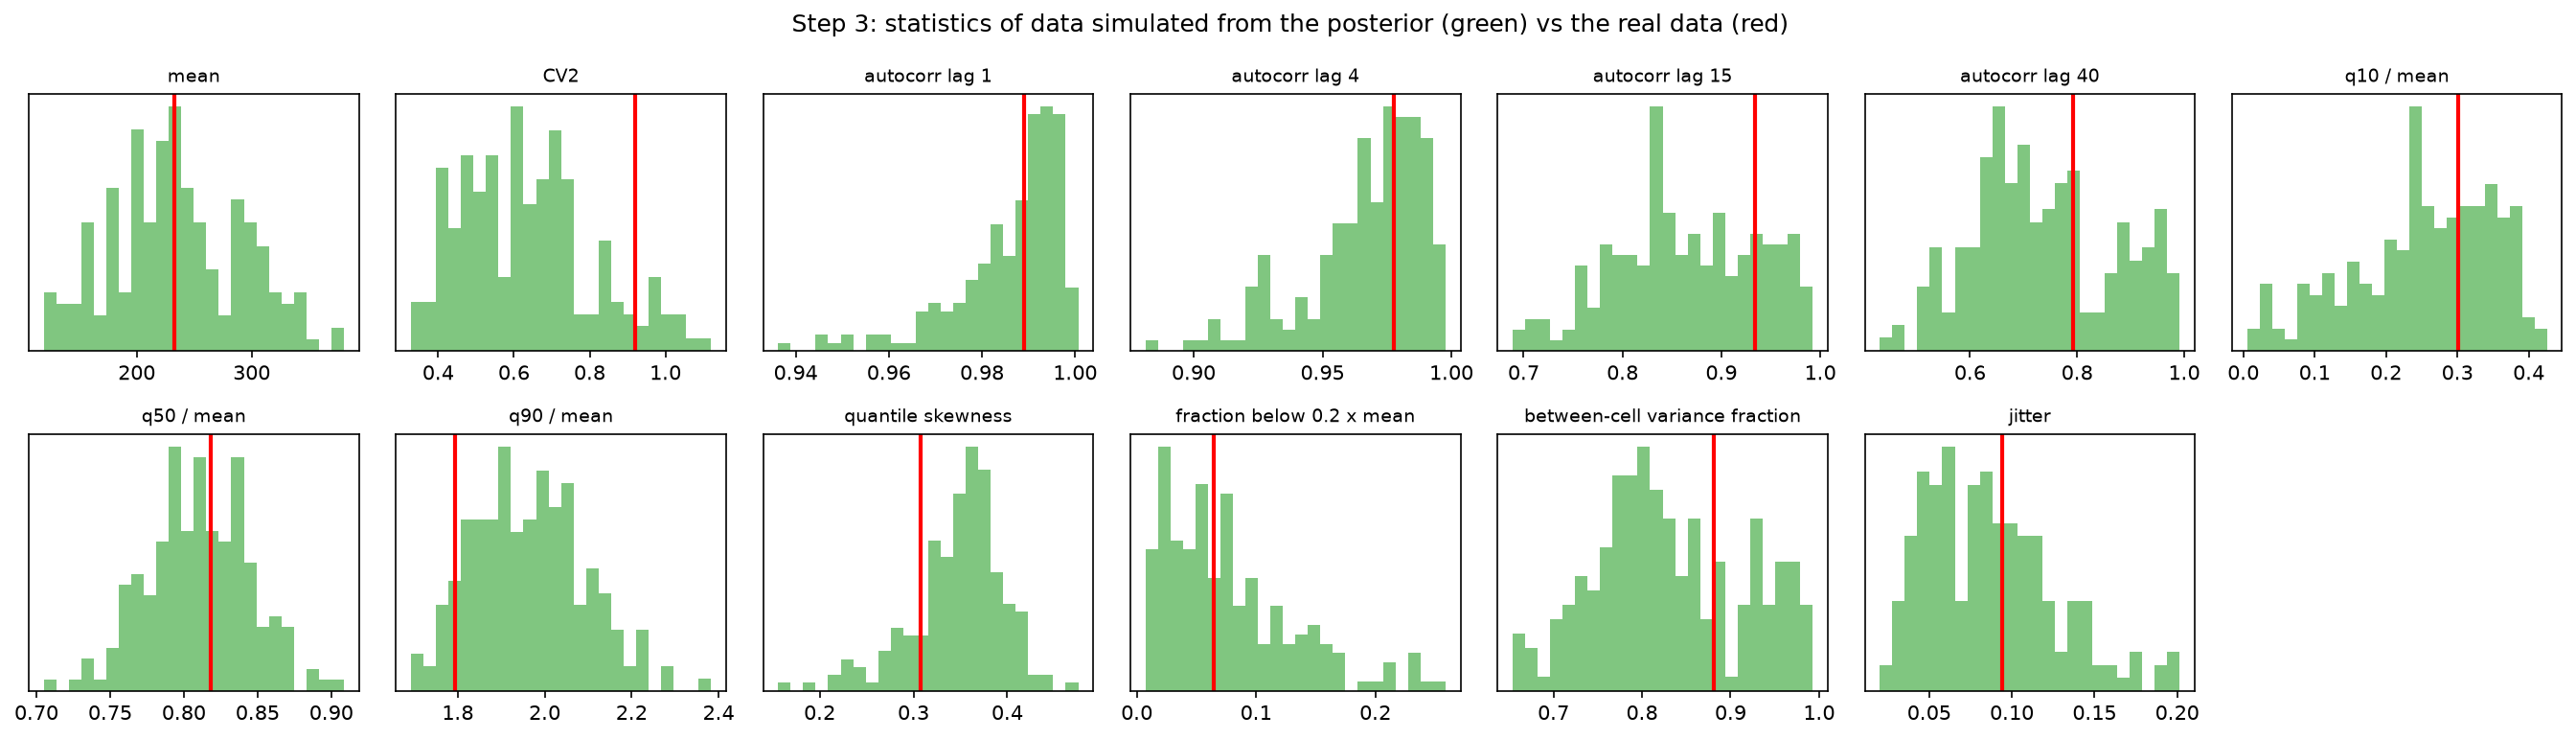
\includegraphics[width=\linewidth]{figures/week4_figure3_ppc.png}
\caption{Posterior predictive.}
\end{figure}

\section{Sensitivity}
\begin{itemize}
  \item drift removal is the big one
\end{itemize}

\begin{figure}[htbp]\centering
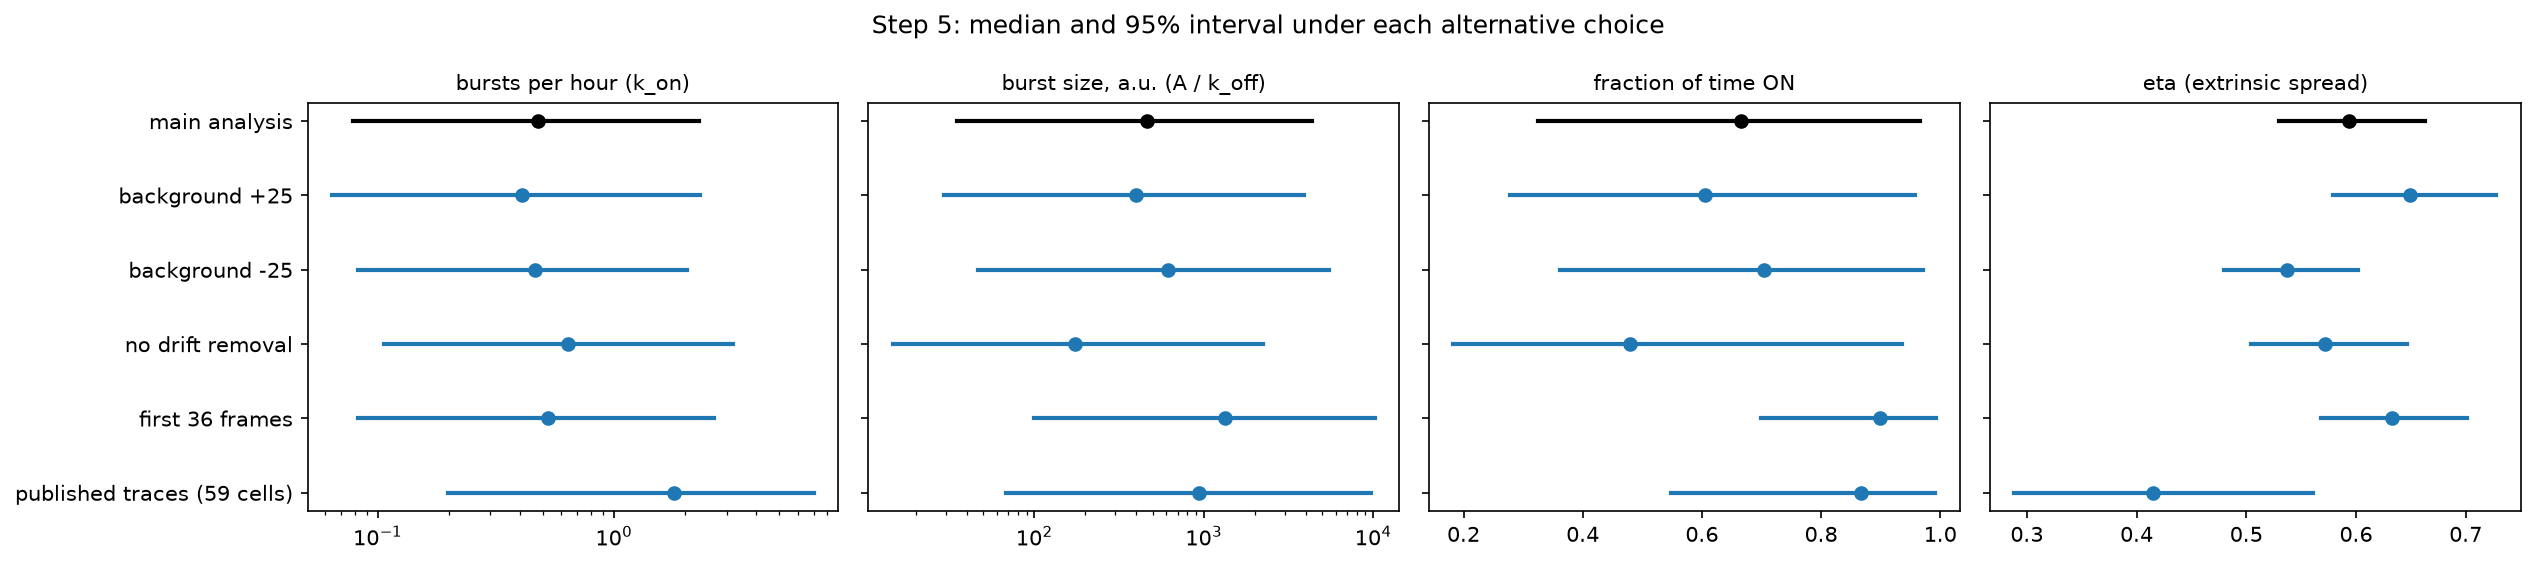
\includegraphics[width=\linewidth]{figures/week4_figure5_sensitivity.png}
\caption{Sensitivity.}
\end{figure}

\section{Held-out tests}
\begin{itemize}
  \item cell split, time split, forecasting
  \item persistence beats the model
  \begin{itemize}
    \item filter works on fake data so it's the model not the code
  \end{itemize}
\end{itemize}

\begin{figure}[htbp]\centering
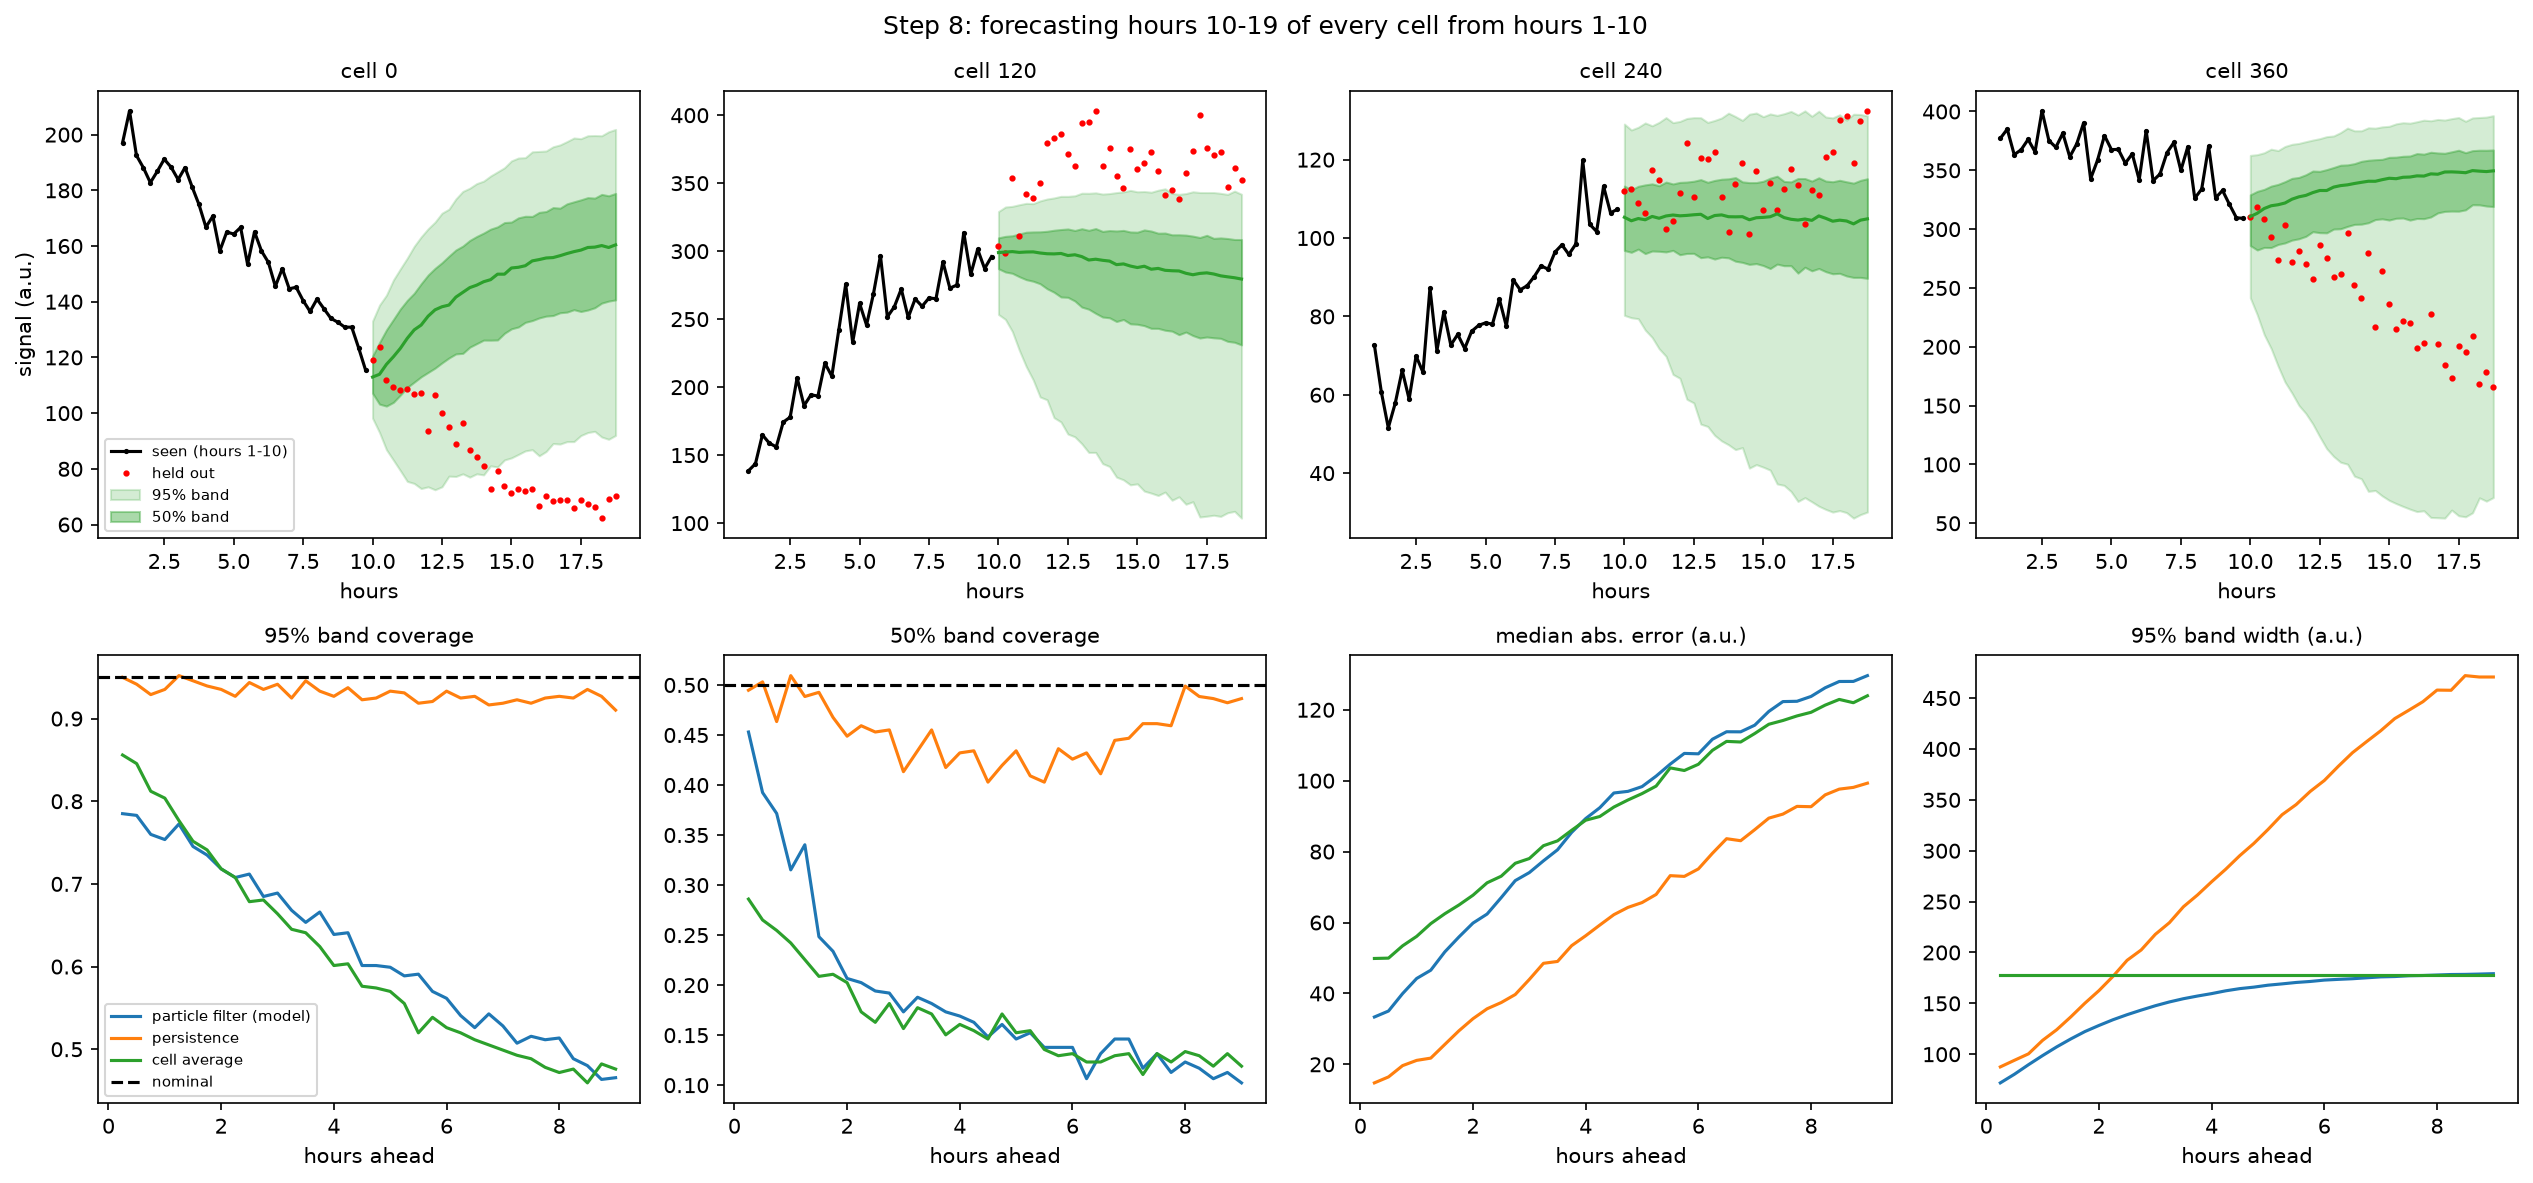
\includegraphics[width=\linewidth]{figures/week4_figure8_forecast.png}
\caption{Forecasting.}
\end{figure}

\section{Comparison with the lab study}
\begin{itemize}
  \item reproduce paper noise numbers \cite{lu2021}
  \item burst frequency matches Dar et al.~\cite{dar2012}
  \begin{itemize}
    \item ON fraction doesn't, explain mRNA thing
  \end{itemize}
\end{itemize}

\begin{figure}[htbp]\centering
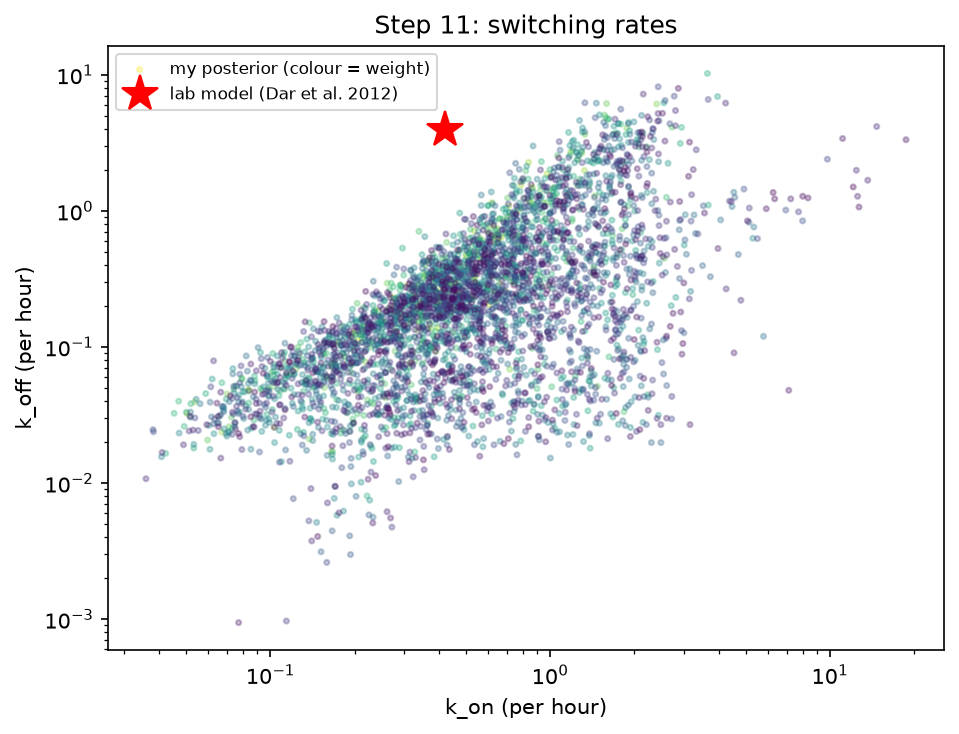
\includegraphics[width=0.6\linewidth]{figures/week4_figure11_switching_rates.png}
\caption{Switching rates vs lab model.}
\end{figure}

\chapter{Discussion}
\begin{itemize}
  \item mostly extrinsic noise
  \item missing Tat feedback / mRNA
  \item one well, drug treated
  \item DNA computing link \cite{soloveichik2010}
  \begin{itemize}
    \item promised this in the proposal, just a paragraph
  \end{itemize}
\end{itemize}

\chapter{Conclusion}

\chapter*{Code availability}
